\IfFileExists{../../_preamble/check_file.tex}% prüfen aus welcher datei der aufruf stattfindet
{%
\providecommand{\myPath}{../../}% file exists=true: befinde mich im unterverzeichnis
}%
{%
\providecommand{\myPath}{}% file exists=false: befinde mich im root_verzeichnis
}%
\documentclass[tikz]{standalone}
%% läd standalone-klasse mit tikz-argument
%//Tikzbibliotheken\\%
\usetikzlibrary{						% Bibliotheken zur direkten Einbindung in TIKZEdt
arrows, 
fit,
shapes.geometric, 
matrix,
calc,
decorations.markings,
decorations.pathreplacing,
decorations.pathmorphing,
backgrounds,
shadings, 
shadows,
positioning,
mindmap,
trees,
datavisualization
}%% diverse tikz-bibliotheken
%%Font etc.%%
\usepackage{lmodern}					% OK, Latin Modern font,											check: 25.08.18
\usepackage{xcolor} 					% OK, Definieren und Nutzen von versch. Farben						check: 25.08.18
\usepackage{graphicx}					% OK, Bereitstellen von \includegraphics							check: 25.08.18

%%Forest%%
\usepackage{forest}						% OK, Baumdarstellung aus dem linguistischen Bereich				check: 25.08.18
\useforestlibrary{edges}

%%Venndiagramm%%
\usepackage{venndiagram}				% OK, Definieren und Darstellen von Venndiagrammen					check: 25.08.18

%%Tabellen%%
\usepackage{booktabs}					% OK, Schönere Tabellen ohne vertikale Linien \toprule etc.			check: 25.08.18
\usepackage{tabularx}					% OK, Weiterer Spaltentyp passt Tabellenbreite  automatisch an		check: 25.08.18
\usepackage{multirow}					% OK, Zellenspannung über mehrere Zeilen							check: 25.08.18
%\usepackage{makecell}					% OK, Tabellenlayout (Tabaellenheader) ähnlich \multirow			check: 25.08.18
\usepackage{tablefootnote}				% OK, Fußnoten in Tabellen (\footnote funktioniert nicht)			check: 25.08.18
\usepackage{array} 						% OK, Erstellen eigener Columntypen in Tabellenumgebungen			check: 25.08.18

%%Grafiken und Plots%%
\usepackage{tikz} 						% OK, Natives zeichnen in Latex ,									check: 25.08.18
\usepackage{tikz-cd} 					% OK, Erstellen von kommutativen Diagrammen in Tikz,				check: 25.08.18
\usepackage{pgfplots}					% OK, Plotten von Daten,											check: 25.08.18
\pgfplotsset{compat=newest}				% OK, Einstellen der Kompatibilitätsversion,						check: 25.08.18
\usepackage{pgfplotstable}				% OK, Plotten und schreiben von Daten in Tabellen,					check: 25.08.18
\usepackage{pgfcalendar} 				% OK, Umrechnen von Datumskoordinaten,								check: 25.08.18
\usepgfplotslibrary{dateplot}			% OK, Plotten von Datumskoordinaten,								check: 25.08.18
\usepgfplotslibrary{units}				% OK, Darstellen von Einheiten als Achsenlabel,						check: 25.08.18%% nur laden wenn weitere graphic pakete benötigt werden (tabellen, pgfplot,...)
%%define tikz-stlyes here, colours etc.
\tikzset{
block_phantom/.style={block_normal, draw=red, fill=none},
block_phantom/.style={block_normal, draw=blue, fill=none}
}
%\tikzstyle{block_phantom}=[block_normal, draw=red, fill=none]%% tikz-styles, farben etc.
\begin{document}%
\IfFileExists{../../_preamble/check_file.tex}% prüfen aus welcher datei der aufruf stattfindet
{%file exists=true: befinde mich im unterverzeichnis
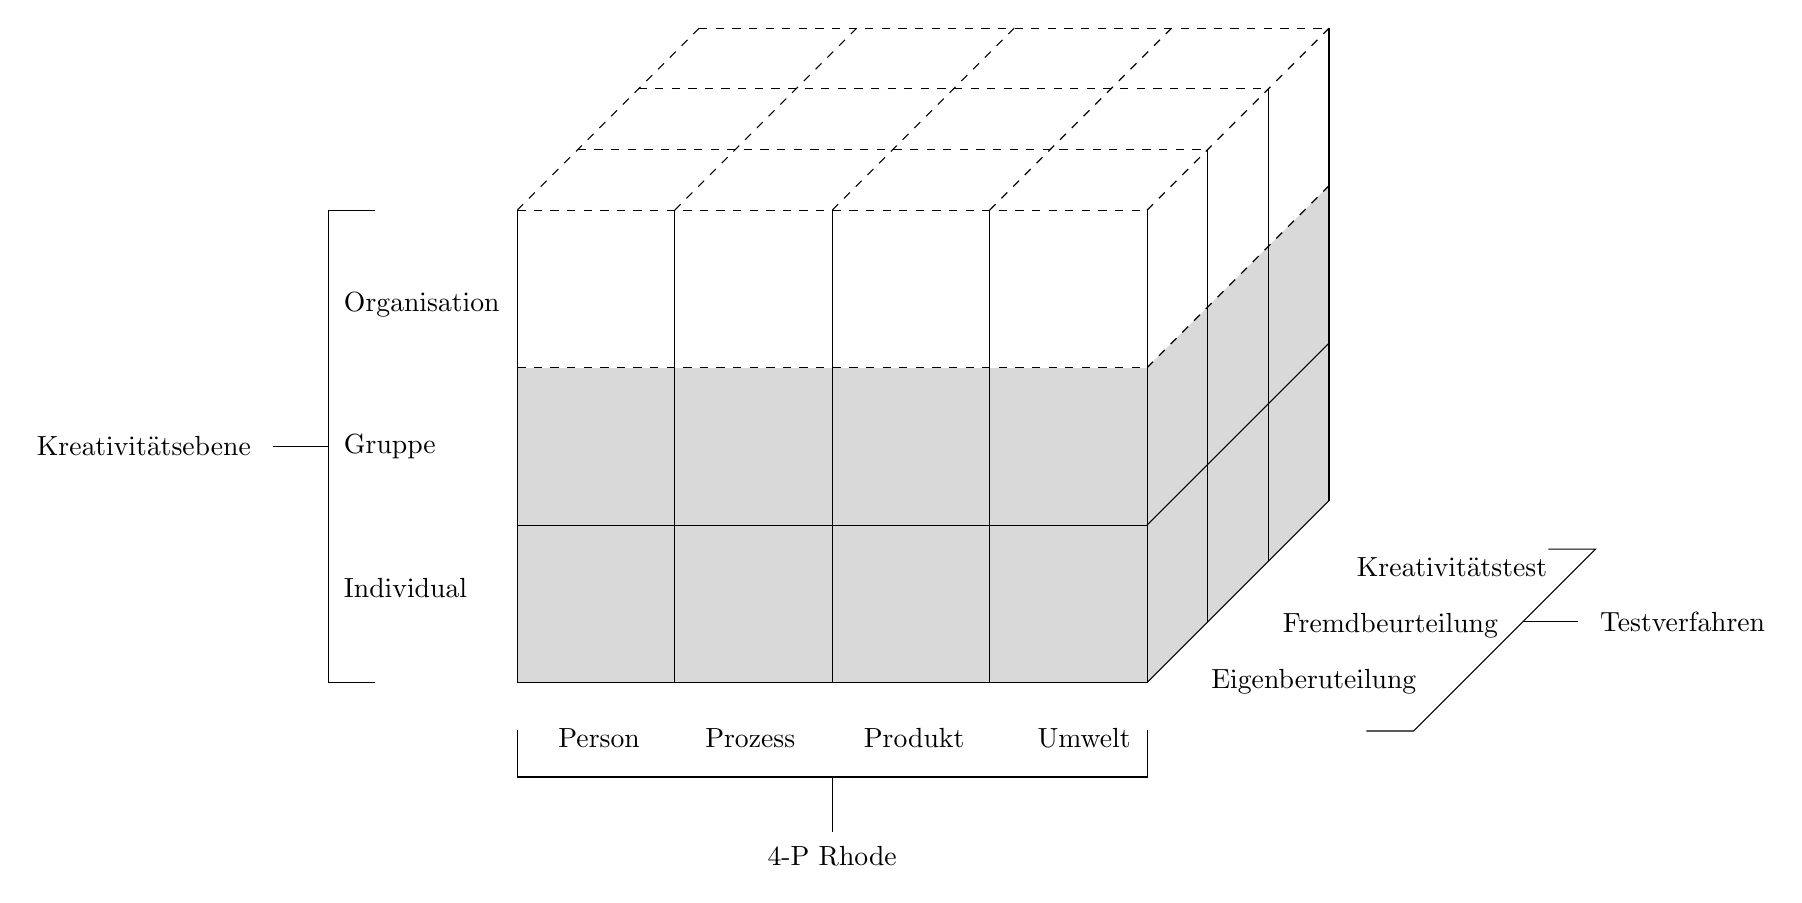
\begin{tikzpicture}[scale=2,every node/.style={scale=1}]

\draw[fill=black!15, draw=none] (0,0,3) rectangle (4,2,3);
\fill[black!15, draw=none] (4 ,0 ,3) -- (4 ,0 ,0) -- (4,2,0) --  (4,2,3) -- cycle;

\foreach \x in {0,...,3} %laenge
{   \draw (\x ,0  ,3 ) -- (\x ,3 ,3 );    
}

\foreach \x in {0,...,4} %laenge
{ 
    \draw [dashed](\x ,3 ,3 ) -- (\x ,3 ,0  );
}


\foreach \x in {0,...,1}
{  \draw (4 ,\x ,3 ) -- (4 ,\x ,0  );
    \draw (0  ,\x ,3 ) -- (4 ,\x ,3 );

}
 \draw [dashed] (4 ,2 ,3 ) -- (4 ,2 ,0  );
 \draw [dashed](0  ,2 ,3 ) -- (4 ,2 ,3 );

\foreach \x in {0,...,3}
{   \draw (4 ,0  ,\x ) -- (4 ,3 ,\x );
    \draw [dashed] (0  ,3 ,\x ) -- (4 ,3 ,\x );
}
%\draw[decorate, decoration={brace, amplitude=.5cm}] (-1,0,3 ) -- node[pos=.5, align=left, xshift=.2cm]{mitte}node[pos=1,xshift=.5cm]{oben}node[pos=0,xshift=.5cm]{unten}node[pos=.5, xshift=-1.7cm, align=right]{beschriftung}(-1,3,3 ); % klammer links
\begin{scope}[text width=2cm, xshift=-.2cm,nodes={draw=none}]
 \draw(-.7,0,3) to (-1,0,3) to 
coordinate[midway] (midleft)
coordinate[midway, xshift=-.7cm] (midleftshift) 
node [midway, xshift=-2.7cm]{Kreativit\"atsebene} 
node [pos=0.2,xshift=1.2cm, align=left]{Individual}
node [pos=.5,xshift=1.2cm, align=left]{Gruppe} 
node [pos=.8,xshift=1.2 cm, align=left]{Organisation}
 (-1,3,3) to (-.7,3,3); %klammer links
 \end{scope}
 \draw (midleft) to (midleftshift);%klammer links


\begin{scope}[text width=1.5cm, yshift=-.1cm, align=center, nodes={draw=none}]
%\draw[decorate, decoration={brace, amplitude=.5cm, mirror}] (0,-.5,3 ) -- node[pos=.5, align=left, yshift=.2cm]{mitte}node[pos=1,yshift=.5cm]{rechts}node[pos=0,yshift=.5cm]{links}node[pos=.5, yshift=-1cm, align=right]{beschriftung}(4,-.5,3 ); %klammer unten
\draw(0,-.2,3) to (0,-.5,3) to 
coordinate[midway] (middown) 
coordinate[midway, yshift=-.7cm] (middownshift) 
node [midway, yshift=-1cm, rotate=0, text width=2cm]{4-P Rhode} 
node [pos=0.13,rotate=0, yshift=.5cm]{Person}
node [pos=0.37,rotate=0,yshift=.5cm]{Prozess} 
node [pos=0.63,rotate=0,yshift=.5cm]{Produkt}  
node [pos=.9,rotate=0,yshift=.5cm]{Umwelt}
(4,-.5,3) to (4,-.2,3); %klammer unten
\end{scope}
\draw (middown) to (middownshift);%klammer unten


%\draw[decorate, decoration={brace, amplitude=.5cm, mirror}] (4,-.5,2.5 ) --  node[pos=.5, align=left, xshift=-.2cm]{mitte}node[pos=1,xshift=-.5cm]{oben}node[pos=0,xshift=-.5cm]{unten}node[pos=.5, xshift=1.7cm, align=right]{beschriftung} (4,-.5,-.5 ); % klammer rechts
\begin{scope}[text width=2.6cm, xshift=1.5cm ,align=left, nodes={draw=none}]
\draw(3.7,-.5,2.5) to (4,-.5,2.5) to 
coordinate[pos=.6] (midright) 
coordinate[pos=.6,xshift=.7cm] (midrightshift) 
node [pos=.9,xshift=-1.5cm]{Kreativit\"atstest} 
node [pos=.58, xshift=-1.7cm]{Fremdbeurteilung}
node [pos=0.1, xshift=-1.5cm, yshift=.4cm]{Eigenberuteilung}
(4,-.5,-.5 ) to (3.7,-.5,-.5); %klammer rechts
\end{scope}
\draw (midright) to node [pos=2.9,xshift=0cm, yshift=0cm, align=left]{Testverfahren} (midrightshift);%klammer rechts


%\draw[red, thick] (4,0,3)--(4,0,0) -- (4,2,0) -- (4,2,3) -- cycle;
%\draw[red, thick] (4,0,3)--(0,0,3)--(0,2,3)--(4,2,3);
\end{tikzpicture}
%
}%
{%file exists=false: befinde mich im root_verzeichnis
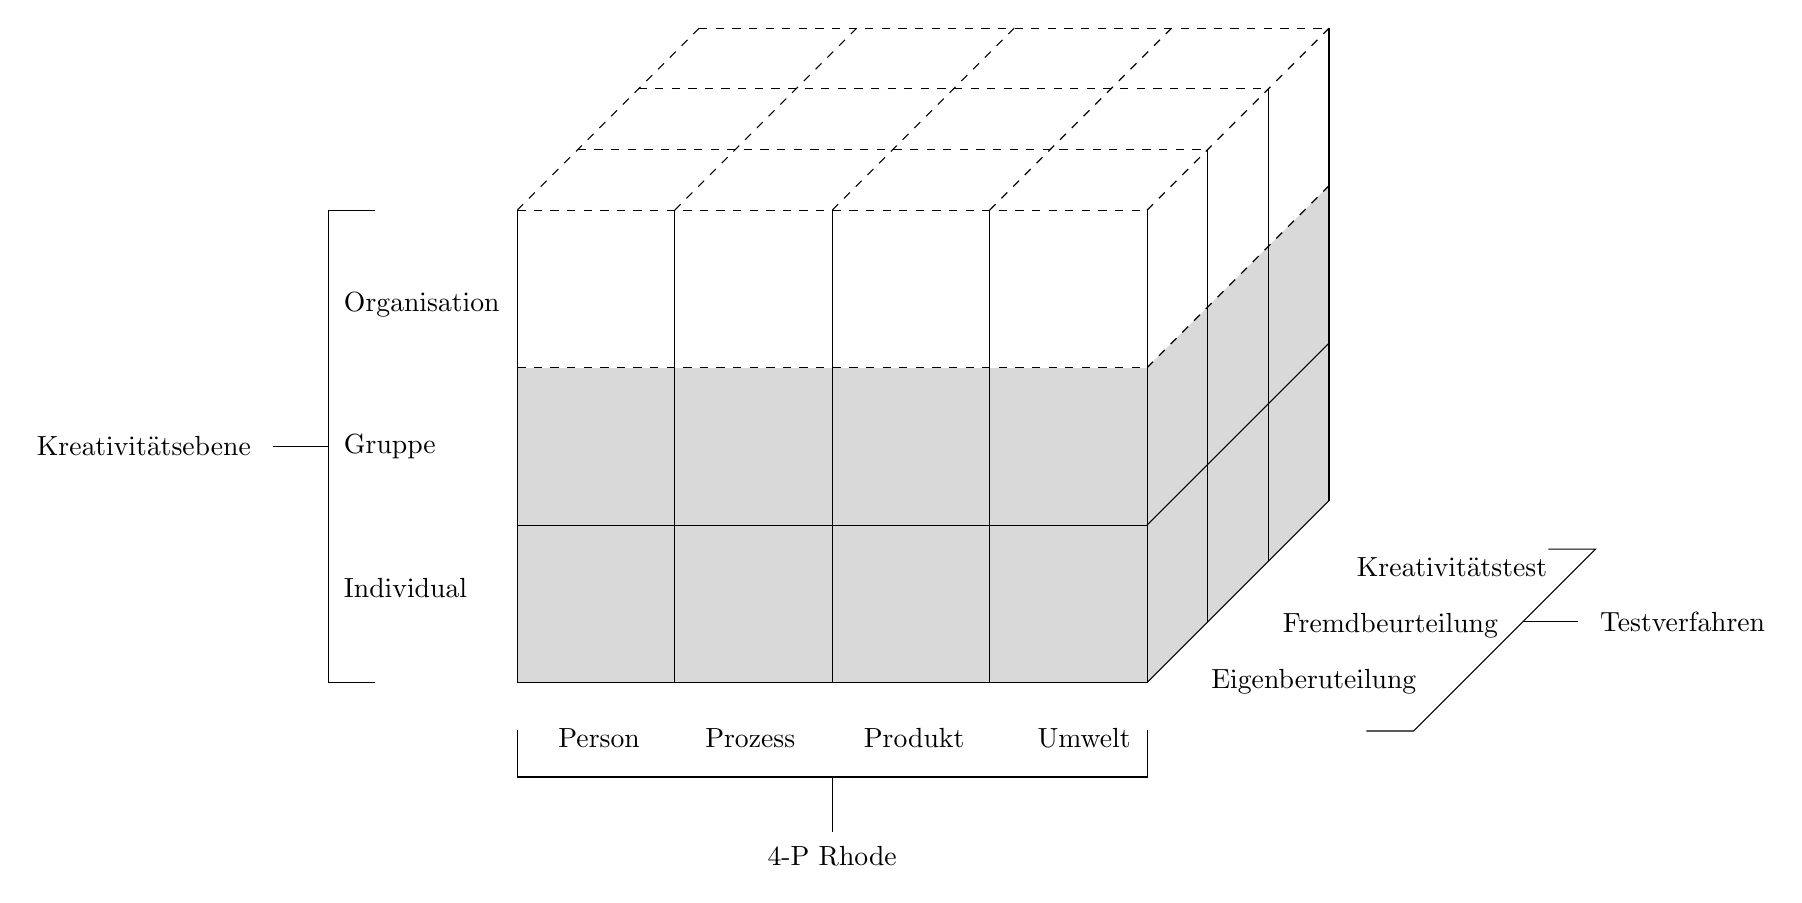
\begin{tikzpicture}[scale=2,every node/.style={scale=1}]

\draw[fill=black!15, draw=none] (0,0,3) rectangle (4,2,3);
\fill[black!15, draw=none] (4 ,0 ,3) -- (4 ,0 ,0) -- (4,2,0) --  (4,2,3) -- cycle;

\foreach \x in {0,...,3} %laenge
{   \draw (\x ,0  ,3 ) -- (\x ,3 ,3 );    
}

\foreach \x in {0,...,4} %laenge
{ 
    \draw [dashed](\x ,3 ,3 ) -- (\x ,3 ,0  );
}


\foreach \x in {0,...,1}
{  \draw (4 ,\x ,3 ) -- (4 ,\x ,0  );
    \draw (0  ,\x ,3 ) -- (4 ,\x ,3 );

}
 \draw [dashed] (4 ,2 ,3 ) -- (4 ,2 ,0  );
 \draw [dashed](0  ,2 ,3 ) -- (4 ,2 ,3 );

\foreach \x in {0,...,3}
{   \draw (4 ,0  ,\x ) -- (4 ,3 ,\x );
    \draw [dashed] (0  ,3 ,\x ) -- (4 ,3 ,\x );
}
%\draw[decorate, decoration={brace, amplitude=.5cm}] (-1,0,3 ) -- node[pos=.5, align=left, xshift=.2cm]{mitte}node[pos=1,xshift=.5cm]{oben}node[pos=0,xshift=.5cm]{unten}node[pos=.5, xshift=-1.7cm, align=right]{beschriftung}(-1,3,3 ); % klammer links
\begin{scope}[text width=2cm, xshift=-.2cm,nodes={draw=none}]
 \draw(-.7,0,3) to (-1,0,3) to 
coordinate[midway] (midleft)
coordinate[midway, xshift=-.7cm] (midleftshift) 
node [midway, xshift=-2.7cm]{Kreativit\"atsebene} 
node [pos=0.2,xshift=1.2cm, align=left]{Individual}
node [pos=.5,xshift=1.2cm, align=left]{Gruppe} 
node [pos=.8,xshift=1.2 cm, align=left]{Organisation}
 (-1,3,3) to (-.7,3,3); %klammer links
 \end{scope}
 \draw (midleft) to (midleftshift);%klammer links


\begin{scope}[text width=1.5cm, yshift=-.1cm, align=center, nodes={draw=none}]
%\draw[decorate, decoration={brace, amplitude=.5cm, mirror}] (0,-.5,3 ) -- node[pos=.5, align=left, yshift=.2cm]{mitte}node[pos=1,yshift=.5cm]{rechts}node[pos=0,yshift=.5cm]{links}node[pos=.5, yshift=-1cm, align=right]{beschriftung}(4,-.5,3 ); %klammer unten
\draw(0,-.2,3) to (0,-.5,3) to 
coordinate[midway] (middown) 
coordinate[midway, yshift=-.7cm] (middownshift) 
node [midway, yshift=-1cm, rotate=0, text width=2cm]{4-P Rhode} 
node [pos=0.13,rotate=0, yshift=.5cm]{Person}
node [pos=0.37,rotate=0,yshift=.5cm]{Prozess} 
node [pos=0.63,rotate=0,yshift=.5cm]{Produkt}  
node [pos=.9,rotate=0,yshift=.5cm]{Umwelt}
(4,-.5,3) to (4,-.2,3); %klammer unten
\end{scope}
\draw (middown) to (middownshift);%klammer unten


%\draw[decorate, decoration={brace, amplitude=.5cm, mirror}] (4,-.5,2.5 ) --  node[pos=.5, align=left, xshift=-.2cm]{mitte}node[pos=1,xshift=-.5cm]{oben}node[pos=0,xshift=-.5cm]{unten}node[pos=.5, xshift=1.7cm, align=right]{beschriftung} (4,-.5,-.5 ); % klammer rechts
\begin{scope}[text width=2.6cm, xshift=1.5cm ,align=left, nodes={draw=none}]
\draw(3.7,-.5,2.5) to (4,-.5,2.5) to 
coordinate[pos=.6] (midright) 
coordinate[pos=.6,xshift=.7cm] (midrightshift) 
node [pos=.9,xshift=-1.5cm]{Kreativit\"atstest} 
node [pos=.58, xshift=-1.7cm]{Fremdbeurteilung}
node [pos=0.1, xshift=-1.5cm, yshift=.4cm]{Eigenberuteilung}
(4,-.5,-.5 ) to (3.7,-.5,-.5); %klammer rechts
\end{scope}
\draw (midright) to node [pos=2.9,xshift=0cm, yshift=0cm, align=left]{Testverfahren} (midrightshift);%klammer rechts


%\draw[red, thick] (4,0,3)--(4,0,0) -- (4,2,0) -- (4,2,3) -- cycle;
%\draw[red, thick] (4,0,3)--(0,0,3)--(0,2,3)--(4,2,3);
\end{tikzpicture}
%
}%
\end{document}%